\chapter{État de l'art sur l'ombrage}
\section{Problématique}


Au vu de l'étude du style, nous voyons que chaque élément visuel suit des règles spécifiques. Donc pour automatiser fidèlement le style il faut automatiser spécifiquement chaque élément. Nous avons vu que l'élément le plus important était l'ombrage, c'est donc sur cet élément visuel que nous allons travailler. 

Ainsi notre contribution à ce travail à été de faire un rendu des ombres le plus fidèle aux panoramas de l'atelier Novat. Notre problématique étant de faire un ombrage de manière a voir la maximum d’éléments sur la surface d'une montagne. Pour ce faire, en plus de nous baser sur le style de l'atelier Novat, nous nous sommes appuyés sur les techniques des cartographes, ainsi que le traitement des ombres non réaliste en informatique graphique. 

\section{L'ombrage vu par les cartographes}

\begin{figure}[!h]
	\centering
 	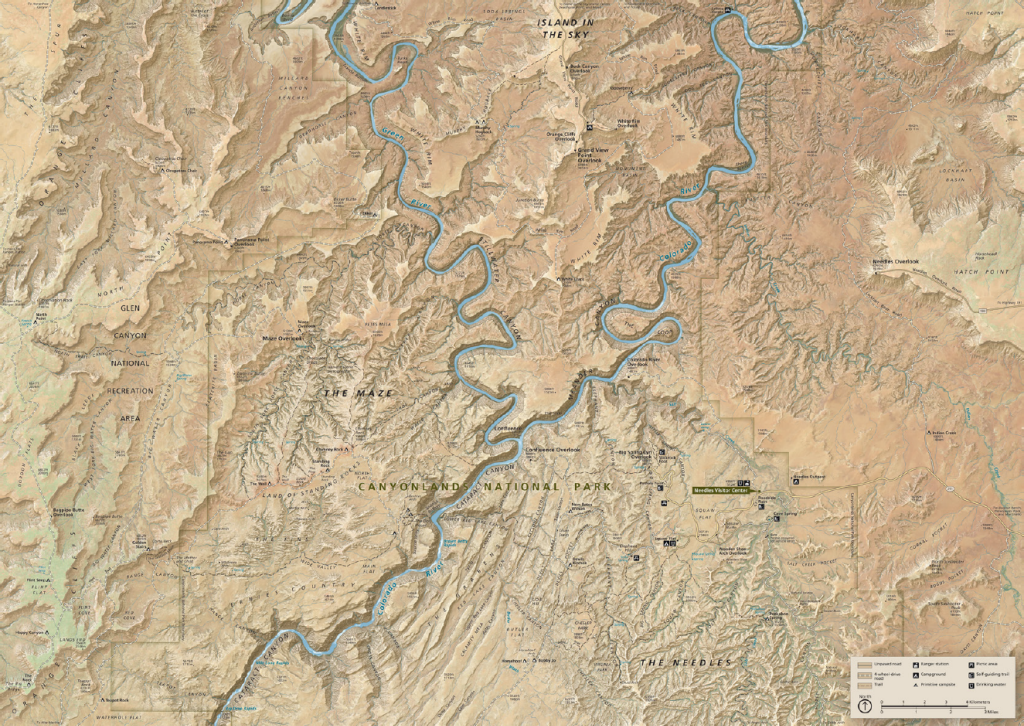
\includegraphics[width=0.7\linewidth]{Etat_de_l_art/carte_Paterson.png}
 	\caption{\textit{The Heart of Canyonlands National Park} par Tom Paterson}
\end{figure}
Pour cette étude, nous nous sommes basés sur les conseils et remarques du cartographe Tom Paterson\footnote{Le site de Tom Paterson où sont référencés tous ses conseils sur l'ombrage de relief : \url{http://www.reliefshading.com/}} \cite{patterson2000view}\cite{patterson2005looking}. Il est important de noter que tous les cartographes n'ont pas la même approche ni le même point de vue sur la façon de faire des cartes. Cependant Tom Paterson reste une référence fiable dans ce domaine.

Que ce soient des cartes vues de dessus ou d'un point vue panoramique, le dessin des ombres est une partie très importante en cartographie. La règle la plus importante est que l'ombrage des reliefs doit décrire la forme du terrain d'une manière descriptive et facilement mesurable. Ainsi la question est : quelles ombres l'artiste doit représenter ? Il y a 2 types d'ombres : l'ombrage et les ombres portées. Si la première ne va qu'assombrir certaines zones, l'autre va projeter la forme d'un élément sur un autre.

Dans la nature, ces deux types sont confondus mais, selon Parterson, uniquement l'ombrage est utilisé en cartographie car les ombres portées peuvent rendre difficile à lire les cartes et peuvent mener à de mauvaise interprétation du terrain. Malgré cela Pierre Novat utilise les ombres portées mais elle sont moins importantes et plus claires que l'ombrage afin de ne pas gêner la lecture. 

Un élément important est de bien définir la direction de la lumière. Même si l'orientation de la lumière par rapport au Nord, que nous appelons azimut, est propre à chaque cartographe, la hauteur (ou élévation), elle, est constante. Elle varie, d'une carte à l'autre, entre $20\degres$ et $50\degres$ mais elle est plus généralement aux alentours de $45\degres$. Une technique essentielle est de réajuster l'azimut de cette lumière localement pour permettre de mieux voir certaines variations de terrain (cf Fig. \ref{fig:corretionLumière}). 


\begin{figure}[!t]
	\centering
 	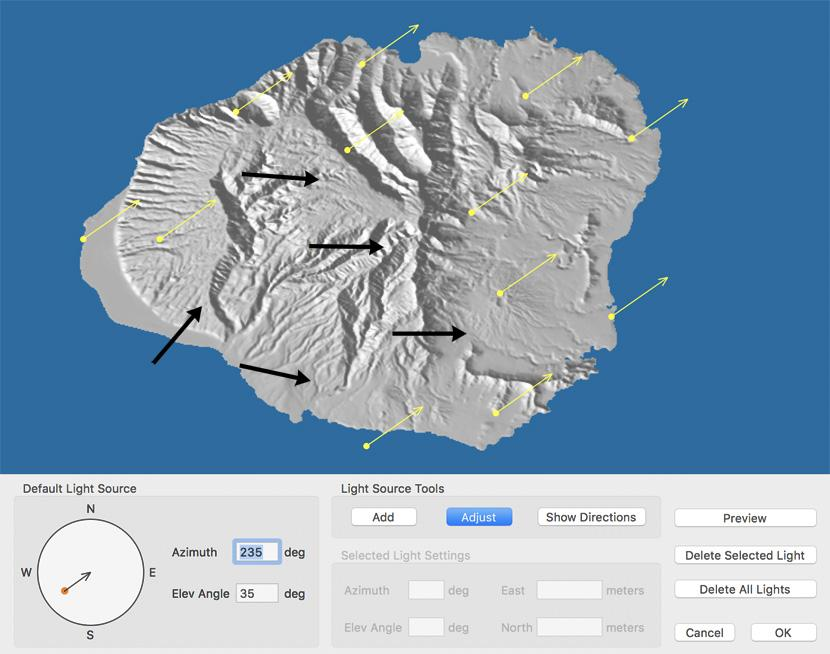
\includegraphics[width=0.7\linewidth]{Etat_de_l_art/multiple_light.jpeg}
 	\caption{\label{fig:corretionLumière}Correction locale de la lumière. Les flèches jaunes représentent la lumière globale, les flèches noires les corrections locales faites par l'artiste.}
\end{figure}

Enfin il existe une autre technique pour améliorer la lecture d'une carte. Le principe est de rendre deux cartes d'ombres. L'une avec un fort contraste, l'autre avec un contraste plus faible pour avoir de meilleurs détails. Ensuite il suffit de les fusionner ensembles avec une interpolation linaire. Cette technique permet d'obtenir les meilleure caractéristiques de chacune. C'est sur ces deux derniers principes que nous baserons notre calcul d'ombrage.




\section{Exagération de la forme en informatique graphique }


La représentation de la forme est une question importante en informatique graphique. Pour pouvoir mieux la percevoir, beaucoup de travaux vont proposer d’exagérer cette forme. Une approche courante est d'utiliser des techniques de rendu à base de lignes pour modifier cette forme. Le principe est d'utiliser la géométrie de l'objet pour ensuite en détecter la forme  en utilisant par exemple la courbure \cite{ohtake2004ridge} et dessiner uniquement les contours de cet objet \cite{zhang2009laplacian}. Seulement, ces techniques ne permettent pas de voir toute les variations d'une forme mais uniquement des zones très localisées comme les crêtes et les vallées. Ainsi utiliser l'ombrage permet de palier à ce problème. 

\paragraph*{Perception de la forme grâce à l'ombrage}
L'ombrage est un élément essentiel en informatique graphique, il permet de percevoir la forme des objets d'une scène et de distinguer leurs détails. Ainsi cette perception peut être manipulée, comme le montrent Vergne et al. dans une étude publiée en 2016 \cite{vergne2016flow} dans laquelle ils modifient l'ombrage des objets pour en modifier la perception. Des études perceptuelles comme celles de Caniard et al. \cite{caniard2007distortion} montrent en effet que l'utilisation d'une unique source lumineuse sur un objet va modifier la perception de cette objet selon la position de souce et donc qu'une unique source de peut pas permettre la perception de toute la forme de l'objet. De plus, dans une étude de 2010, Lopez et al.~\cite{lopez2010measuring} font l'expérience suivante : dans une scène où 0, 1 ou 2 objets sur 6 objets, sont éclairés avec un angle de lumière différent, ils demandent à des sujets de les identifier. Le résultat montre que le cerveau humain n'arrive pas à percevoir cette différence d'angle. Ainsi l'ensemble de ces études montrent que 1: la direction de la lumière est primordiale pour bien percevoir la forme d'un objet et 2: notre perception visuelle a bien du mal à estimer la direction de la lumière. Nous pouvons donc modifier celle ci pour mettre en valeur le relief, tout en conservant une cohérence globale.

\paragraph*{Modification de l'ombrage}
Pour augmenter la perception de la forme grâce à l'ombrage, il existe plusieurs approches. Une technique très utilisée est celle de l’occlusion ambiante proposée par Pharr et Green \cite{pharr2004ambient}. En se basant sur une technique introduite par Miller et al. \cite{miller1994efficient} qui permet de détecter les cavités sur une surface 3D, ils les utilisent pour modifier localement l'ombrage et ainsi faire mieux ressortir ces cavités. Cette méthode a néanmoins tendance à faire ressortir uniquement les cavités profondes tout en lissant les moins profondes. Une autre approche proposée par Ritshel et al. \cite{ritschel20083d} est d'utiliser l'illusion de Cornsweet pour créer un masque qu'il applique sur un ombrage classique. Le problème est que cela va augmenter les contrastes si un flan de montagne est vraiment dans l'ombre et donc cela ne permet pas de "déboucher" les ombres. 

Une autre solution publiée par Zhang et al. \cite{zhang2010perceptually} est d'uniquement modifier la normale à l'aide de la courbure de l'objet de manière à optimiser la perception des aspérités de l'objet.
Un travail similaire publié par Vergne et al. \cite{vergne2008apparent} propose un ombrage uniquement basé sur la courbure d'un objet. À cette courbure ils assignent une carte de relief, c'est-à-dire que pour chaque valeur de courbure ils associent une valeur d'ombre comprise entre $0$ et $1$. Le problème de ces 2 approches c'est qu'en plus de ne pas avoir de lumière globale, elles utilisent la courbure qui en cartographie n'est pas une information pertinente pour calculer un ombrage qui met en valeur les montagnes. Dans notre approche nous utiliserons plutôt la pente.

\paragraph*{Exagerated Shading}
Une technique introduite par Rusinkiewicz et al. \cite{rusinkiewicz2006exaggerated} et plus proche de notre solution est d’exagérer l'ombrage afin d'avoir une meilleure perception des aspérités d'une surface. Le principe est de faire un ombrage sur plusieurs échelles, chaque échelle ayant un niveau de flou différent. Pour chaque échelle, ils modifient la hauteur de la lumière avant de calculer un nouvel ombrage. Ensuite ils somment toutes les échelles pour obtenir le rendu final (Fig. \ref{fig:exageratedShading}).  Leur approche est assez intéressante car elle a été construite à partir des règles de cartographie de Tom Paterson. En effet son but premier est de s'approcher au mieux de l'ombrage des cartes vues de dessus.  


\begin{figure*}[h!]
\centering
 \begin{subfigure}[t]{0.47\textwidth}
 \centering
 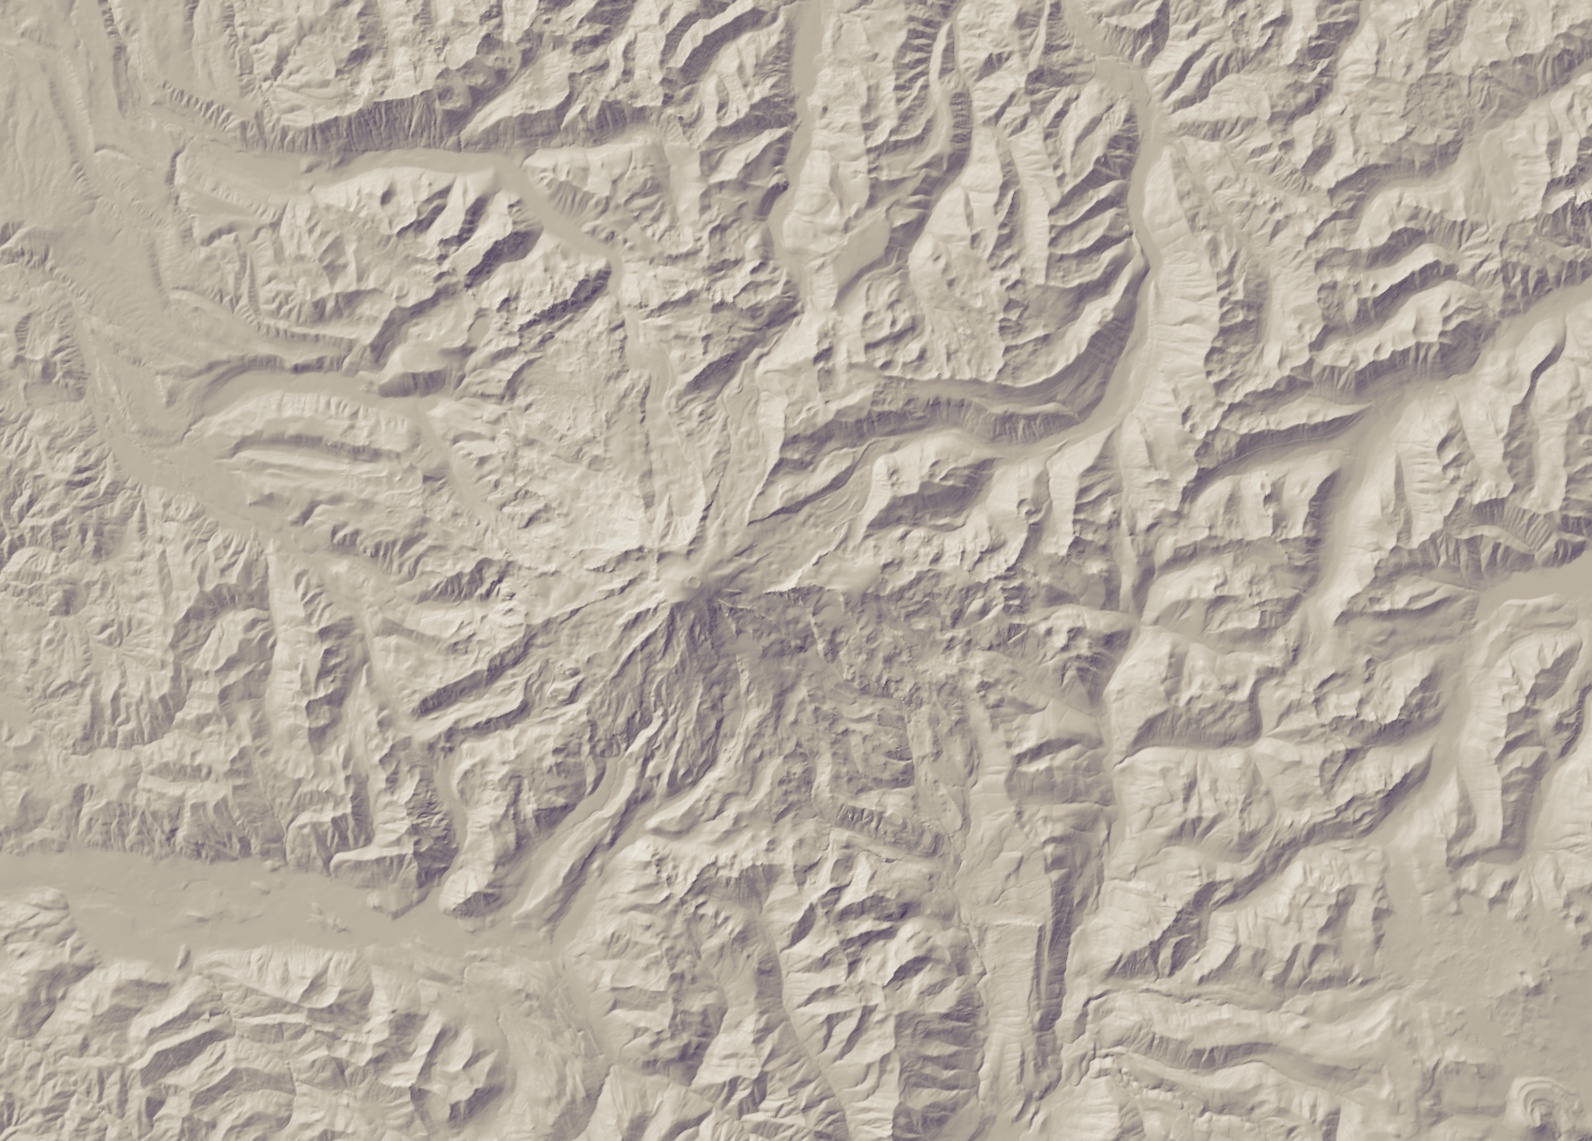
\includegraphics[width=1.0\linewidth]{Etat_de_l_art/terrain_diffuse.jpg}
 \caption{Ombrage classique}
 \end{subfigure}%
 ~
 \hspace{.05\textwidth}
 \begin{subfigure}[t]{0.47\textwidth}
 \centering
 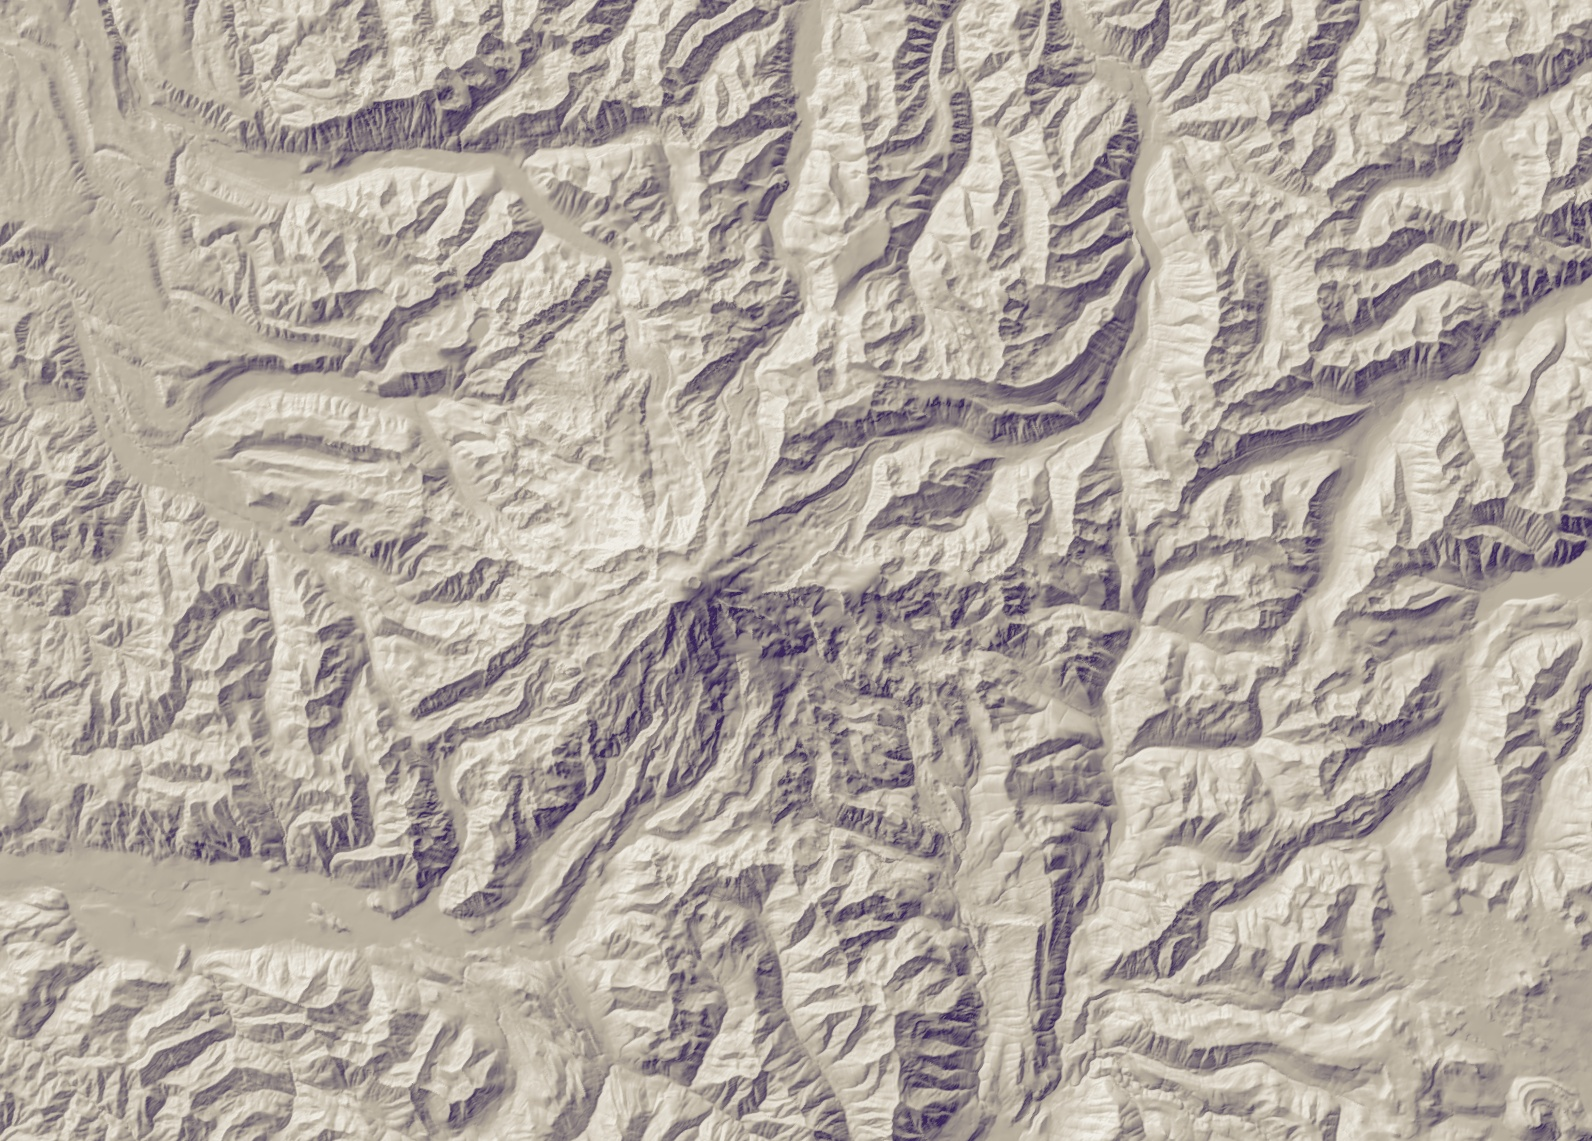
\includegraphics[width=1.0\linewidth]{Etat_de_l_art/terrain_exag.jpg}
 \caption{\textit{Exagerated Shading}}
 \end{subfigure}
 \caption{\label{fig:exageratedShading} Méthode de l'\textit{Exagerated Shading} sur un terrain montagneux}
\end{figure*}

Le principal inconvénient avec cette technique c'est qu'elle donne un effet bas-relief au rendu. Notre solution est inspirée de leur approche mais plus adaptée à un format panorama. 


\paragraph*{La Couleur} Une fois l'intensité de l'ombrage connue, il faut une méthode pour la dessiner. La technique la plus classique est de simplement multiplier cette intensité par la couleur de l'objet. Une approche plus complète serait d'utiliser une technique dite de "mélange" comme par exemple celle utilisée par Bousseau et al. \cite{bousseau2006interactive}  pour faire une rendu type aquarelle qui introduit notamment une fonction pour étendre une couleur sur une rampe  à l'aide d'une intensité (Fig. \ref{fig:watercolorschema}).
Une autre approche est d'associer cette intensité à une texture 1D de couleur. Cette texture peut être continue ou discontinue (technique du \textit{cel-shading}) permettant d'obtenir des contours très marqués et de donner un aspect "cartoon". 

Pour étendre le degré de contrôle du rendu de l'ombrage Barla et al. \cite{barla2006x} proposent d'utiliser une texture 2D dont l’abscisse donne la couleur correspondant à une intensité donnée (comme pour la texture de couleur 1D) et dont l'ordonnée peut être liée à n’importe quel autre paramètre de la scène (Fig. \ref{fig:xtoontexture}). Une telle approche pourrait permettre de prendre en compte par exemple la distance au point de vue ou l'altitude dans un rendu de panorama.

\begin{figure}[h!]
    \begin{minipage}[b]{0.4\linewidth}
        \centering 
        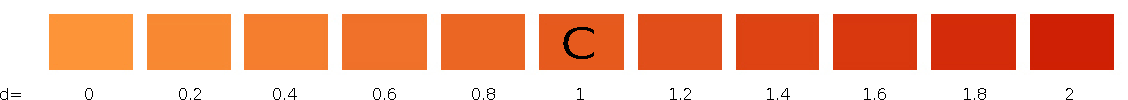
\includegraphics[width=1.0\linewidth]{Etat_de_l_art/watercolor.pdf}
        \caption{\label{fig:watercolorschema} Éclaircissement et assombrissement de la couleur $C$ (ici $(0.90,0.35,0.12)$) en utilisant le paramètre de densité $d$ \cite{bousseau2006interactive}.}

    \end{minipage}\hfill
    \begin{minipage}[b]{0.40\linewidth}
        \centering 
        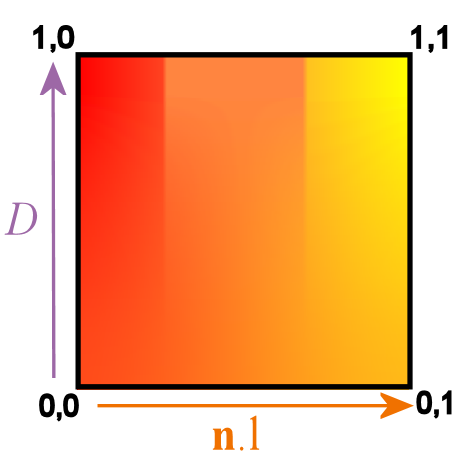
\includegraphics[width=0.5\linewidth]{Etat_de_l_art/xToon.png}
 		\caption{\label{fig:xtoontexture} Une texture 2D avec $l.n$ en paramètre principal et $D$ comme paramètre secondaire \cite{barla2006x}. }
    \end{minipage}
\end{figure}




